\chapter{}

%\begin{longtblr}[
%	caption = {Indicadores Estatísticos referentes ao número de entidades concorrentes em concursos públicos por CPV : R019},
%	label = {tab:test},
%	]{
%		colspec = {|c|c|c|c|c|c|c|c|c|c|},
%		rowhead = 1,
%		hlines,
%		%row{even} = {gray9},
%		%row{1} = {olive9},
%	} 
%		\textbf{CPV} & \textbf{NEC Total} & \textbf{Nº Concursos} & \textbf{Média}     & \textbf{$\sigma$}  & \textbf{Mínimo} & \textbf{Q1} & \textbf{Q2} & \textbf{Q3} & \textbf{Máximo} \\  
%		98           & 1739               & 586                   & 2.967              & 2.251 & 1               & 1           & 2           & 4           & 15              \\ 
%		92           & 2127               & 680                   & 3.127 			   & 2.501 & 1               & 1           & 3           & 4           & 18              \\ 
%		90           & 27135              & 4031                  & 6.731 			   & 4.878 & 1               & 3           & 6           & 9           & 27              \\ 
%		85           & 4497               & 1231                  & 3.653 			   & 2.810 & 1               & 1           & 3           & 5           & 18              \\ 
%		80           & 1812               & 495                   & 3.660 			   & 3.362 & 1               & 1           & 3           & 5           & 32              \\ 
%		79           & 20469              & 3678                  & 5.565 			   & 4.006 & 1               & 2           & 5           & 8           & 30              \\ 
%		77           & 13301              & 1528                  & 8.704 			   & 6.449 & 1               & 4           & 8           & 12          & 33              \\ 
%		76           & 64                 & 28                    & 2.285 			   & 1.560 & 1               & 1           & 1.5         & 3.25        & 6               \\ 
%		75           & 606                & 134                   & 4.522 			   & 4.179 & 1               & 1           & 3           & 6           & 21              \\ 
%		73           & 598                & 121                   & 4.942 			   & 6.532 & 1               & 1           & 3           & 6           & 32              \\ 
%		72           & 12662              & 3080                  & 4.111 			   & 4.807 & 1               & 1           & 2           & 5           & 32              \\ 
%		71           & 27396              & 3430                  & 7.987 			   & 7.420 & 1               & 3           & 6           & 11          & 54              \\ 
%		70           & 111                & 40                    & 2.775 			   & 3.050 & 1               & 1           & 1           & 2.25        & 14              \\ 
%		66           & 11105              & 2792                  & 3.977 			   & 2.132 & 1               & 2           & 4           & 6           & 11              \\ 
%		65           & 1476               & 339                   & 4.353 			   & 2.864 & 1               & 2           & 4           & 6           & 12              \\ 
%		64           & 2379               & 962                   & 2.472 			   & 1.588 & 1               & 2           & 2           & 3           & 29              \\ 
%		63           & 7115               & 831                   & 8.561 			   & 6.509 & 1               & 2           & 8           & 14          & 24              \\ 
%		60           & 12889              & 2930                  & 4.398 			   & 3.443 & 1               & 1           & 4           & 6           & 27              \\ 
%		55           & 7394               & 1365                  & 5.416 			   & 7.699 & 1               & 2           & 4           & 5           & 46              \\ 
%		51           & 475                & 193                   & 2.461 			   & 1.851 & 1               & 1           & 2           & 3           & 12              \\ 
%		50           & 17208              & 3187                  & 5.399 			   & 7.272 & 1               & 2           & 3           & 6           & 40              \\ 
%		48           & 5520               & 1717                  & 3.214 			   & 3.300 & 1               & 1           & 2           & 4           & 19              \\ 
%		45           & 103881             & 17913                 & 5.799 			   & 4.428 & 1               & 3           & 5           & 8           & 38              \\ 
%		44           & 8598               & 2123                  & 4.049 			   & 2.879 & 1               & 2           & 4           & 5.5         & 20              \\ 
%		43           & 988                & 239                   & 4.133 			   & 3.556 & 1               & 2           & 3           & 5           & 15              \\ 
%		42           & 4178               & 989                   & 4.224 			   & 3.524 & 1               & 2           & 3           & 5           & 22              \\ 
%		41           & 14                 & 3                     & 4.666 			   & 3.511 & 1               & 3           & 5           & 6.5         & 8               \\ 
%		39           & 18888              & 2673                  & 7.066 			   & 5.431 & 1               & 3           & 6           & 10          & 37              \\ 
%		38           & 9390               & 1254                  & 7.488 			   & 7.428 & 1               & 2           & 4           & 11          & 33              \\ 
%		37           & 777                & 195                   & 3.984 			   & 2.512 & 1               & 2           & 4           & 5           & 12              \\ 
%		35           & 6221               & 876                   & 7.101 			   & 7.613 & 1               & 3           & 5           & 9           & 47              \\ 
%		34           & 13432              & 3736                  & 3.595 			   & 2.682 & 1               & 2           & 3           & 5           & 19              \\ 
%		33           & 265993             & 23180                 & 11.47 			   & 9.472 & 1               & 4           & 9           & 16          & 65              \\ 
%		32           & 4316               & 1008                  & 4.281 			   & 3.432 & 1               & 2           & 3           & 6           & 21              \\ 
%		31           & 3632               & 748                   & 4.855 			   & 3.633 & 1               & 2           & 4           & 6           & 27              \\ 
%		30           & 30955              & 4393                  & 7.046 			   & 4.863 & 1               & 3           & 6           & 10          & 21              \\ 
%		24           & 3971               & 846                   & 4.693 			   & 5.198 & 1               & 2           & 3           & 5           & 39              \\ 
%		22           & 2196               & 544                   & 4.036 			   & 3.075 & 1               & 2           & 3           & 5           & 25              \\ 
%		19           & 1093               & 292                   & 3.743 			   & 2.160 & 1               & 2           & 4           & 5           & 13              \\ 
%		18           & 8730               & 982                   & 8.890 			   & 8.402 & 1               & 4           & 7           & 12          & 53              \\ 
%		16           & 788                & 190                   & 4.147 			   & 2.954 & 1               & 2           & 3           & 6           & 13              \\ 
%		15           & 26523              & 4749                  & 5.584 			   & 5.137 & 1               & 2           & 4           & 8           & 30              \\ 
%		14           & 752                & 245                   & 3.069 			   & 1.837 & 1               & 2           & 3           & 4           & 10              \\ 
%		09           & 9086               & 2392                  & 3.798 			   & 2.410 & 1               & 2           & 3           & 5           & 27              \\ 
%		03           & 2915               & 661                   & 4.409 			   & 4.044 & 1               & 2           & 3           & 6           & 30              \\ 
%		00           & 136                & 107                   & 1.271 			   & 1.120 & 1               & 1           & 1           & 1           & 6               \\ 
%\end{longtblr}


%\begin{longtable}{@{} *{11}{>{\centering\arraybackslash}X} @{}} % Adjust the number of columns
%	\caption{Indicadores Estatísticos referentes ao número de entidades concorrentes em concursos públicos por CPV e por Tipo de Contrato : R019}
%	\label{tab:test} 
%	\toprule
%	\textbf{CPV} & \textbf{Tipo de Contrato} & \textbf{NEC Total} & \textbf{Nº Concursos} & \textbf{Média} & \textbf{$\sigma$} & \textbf{Min} & \textbf{Q1} & \textbf{Q2} & \textbf{Q3} & \textbf{Máx} \\
%	\midrule
%	\endfirsthead
%	
%	\multicolumn{11}{c}%
%	{\tablename\ \thetable\ -- \textit{Continued from previous page}} \\
%	\toprule
%	\textbf{CPV} & \textbf{Tipo de Contrato} & \textbf{NEC Total} & \textbf{Nº Concursos} & \textbf{Média} & \textbf{$\sigma$} & \textbf{Min} & \textbf{Q1} & \textbf{Q2} & \textbf{Q3} & \textbf{Máx} \\
%	\midrule
%	\endhead
%	
%	\midrule \multicolumn{11}{r}{\textit{Continued on next page}} \\
%	\endfoot
%	
%	\bottomrule
%	\endlastfoot
%    
%	   
%			98  & Bens e Serviços                       & 1723      & 581          & 2.966  & 2.244    & 1   & 1    & 2   & 4    & 15  \\  
%			98  & Empreitadas                           & 4         & 2            & 2.000  & 1.414    & 1   & 1.5  & 2   & 2.5  & 3   \\  
%			98  & Outro                                 & 12        & 3            & 4.000  & 4.359    & 1   & 1.5  & 2   & 5.5  & 9   \\  
%			92  & Bens e Serviços                       & 2126      & 679          & 3.131  & 2.502    & 1   & 1    & 3   & 4    & 18  \\  
%			92  & Empreitadas                           & 1         & 1            & 1.000  & NaN      & 1   & 1    & 1   & 1    & 1   \\  
%			90  & Bens e Serviços                       & 27135     & 4031         & 6.732  & 4.878    & 1   & 3    & 6   & 9    & 27  \\  
%			85  & Bens e Serviços                       & 4496      & 1230         & 3.655  & 2.811    & 1   & 1    & 3   & 5    & 18  \\  
%			85  & Empreitadas                           & 1         & 1            & 1.000  & NaN      & 1   & 1    & 1   & 1    & 1   \\  
%			80  & Bens e Serviços                       & 1812      & 495          & 3.661  & 3.363    & 1   & 1    & 3   & 5    & 32  \\  
%			79  & Bens e Serviços                       & 20464     & 3677         & 5.565  & 4.007    & 1   & 2    & 5   & 8    & 30  \\  
%			79  & Outro                                 & 5         & 1            & 5.000  & NaN      & 5   & 5    & 5   & 5    & 5   \\  
%			77  & Bens e Serviços                       & 13300     & 1527         & 8.710  & 6.448    & 1   & 4    & 8   & 12   & 33  \\  
%			77  & Empreitadas                           & 1         & 1            & 1.000  & NaN      & 1   & 1    & 1   & 1    & 1   \\  
%			76  & Bens e Serviços                       & 64        & 28           & 2.286  & 1.560    & 1   & 1    & 1.5 & 3.25 & 6   \\  
%			75  & Bens e Serviços                       & 606       & 134          & 4.522  & 4.180    & 1   & 1    & 3   & 6    & 21  \\  
%			73  & Bens e Serviços                       & 598       & 121          & 4.942  & 6.532    & 1   & 1    & 3   & 6    & 32  \\  
%			72  & Bens e Serviços                       & 12662     & 3080         & 4.111  & 4.808    & 1   & 1    & 2   & 5    & 32  \\  
%			71  & Bens e Serviços                       & 27341     & 3418         & 7.999  & 7.428    & 1   & 3    & 6   & 11   & 54  \\  
%			71  & Empreitadas                           & 55        & 12           & 4.583  & 3.825    & 1   & 1.75 & 4   & 4.75 & 14  \\  
%			70  & Bens e Serviços                       & 111       & 40           & 2.775  & 3.051    & 1   & 1    & 1   & 2.25 & 14  \\  
%			66  & Bens e Serviços                       & 11105     & 2792         & 3.977  & 2.132    & 1   & 2    & 4   & 6    & 11  \\  
%			65  & Bens e Serviços                       & 1476      & 339          & 4.354  & 2.865    & 1   & 2    & 4   & 6    & 12  \\  
%			64  & Bens e Serviços                       & 2379      & 962          & 2.473  & 1.589    & 1   & 2    & 2   & 3    & 29  \\  
%			63  & Bens e Serviços                       & 7115      & 831          & 8.562  & 6.510    & 1   & 2    & 8   & 14   & 24  \\  
%			60  & Bens e Serviços                       & 12886     & 2929         & 4.399  & 3.444    & 1   & 1    & 4   & 6    & 27  \\  
%			60  & Outro                                 & 3         & 1            & 3.000  & NaN      & 3   & 3    & 3   & 3    & 3   \\  
%			55  & Bens e Serviços                       & 7376      & 1356         & 5.440  & 7.719    & 1   & 2    & 4   & 5    & 46  \\  
%			55  & Outro                                 & 18        & 9            & 2.000  & 1.658    & 1   & 1    & 1   & 2    & 6   \\  
%			51  & Bens e Serviços                       & 475       & 193          & 2.461  & 1.851    & 1   & 1    & 2   & 3    & 12  \\  
%			50  & Bens e Serviços                       & 17153     & 3172         & 5.408  & 7.286    & 1   & 2    & 3   & 6    & 40  \\  
%			50  & Empreitadas                           & 55        & 15           & 3.667  & 3.155    & 1   & 1    & 2   & 6.5  & 10  \\  
%			48  & Bens e Serviços                       & 5520      & 1717         & 3.215  & 3.301    & 1   & 1    & 2   & 4    & 19  \\  
%			45  & Empreitadas                           & 103881    & 17913        & 5.799  & 4.429    & 1   & 3    & 5   & 8    & 38  \\  
%			44  & Bens e Serviços                       & 8598      & 2123         & 4.050  & 2.880    & 1   & 2    & 4   & 5.5  & 20  \\  
%			43  & Bens e Serviços                       & 988       & 239          & 4.134  & 3.556    & 1   & 2    & 3   & 5    & 15  \\  
%			42  & Bens e Serviços                       & 4164      & 985          & 4.227  & 3.531    & 1   & 2    & 3   & 6    & 22  \\  
%			42  & Empreitadas                           & 14        & 4            & 3.500  & 1.000    & 2   & 3.5  & 4   & 4    & 4   \\  
%			41  & Bens e Serviços                       & 14        & 3            & 4.667  & 3.512    & 1   & 3    & 5   & 6.5  & 8   \\  
%			39  & Bens e Serviços                       & 18881     & 2669         & 7.074  & 5.432    & 1   & 3    & 6   & 10   & 37  \\  
%			39  & Empreitadas                           & 7         & 4            & 1.750  & 0.957    & 1   & 1    & 1.5 & 2.25 & 3   \\  
%			38  & Bens e Serviços                       & 9387      & 1251         & 7.504  & 7.431    & 1   & 2    & 4   & 11   & 33  \\  
%			38  & Empreitadas                           & 3         & 3            & 1.000  & 0.000    & 1   & 1    & 1   & 1    & 1   \\  
%			37  & Bens e Serviços                       & 777       & 195          & 3.985  & 2.513    & 1   & 2    & 4   & 5    & 12  \\  
%			35  & Bens e Serviços                       & 6209      & 875          & 7.096  & 7.616    & 1   & 3    & 5   & 9    & 47  \\  
%			35  & Empreitadas                           & 12        & 1            & 12.000 & NaN      & 12  & 12   & 12  & 12   & 12  \\  
%			34  & Bens e Serviços                       & 13336     & 3730         & 3.575  & 2.628    & 1   & 2    & 3   & 5    & 17  \\  
%			34  & Empreitadas                           & 96        & 6            & 16.000 & 6.419    & 3   & 17.5 & 19  & 19   & 19  \\ 
%			33  & Bens e Serviços                       & 265988    & 23179        & 11.475 & 9.473    & 1   & 4    & 9   & 16   & 65  \\  
%			33  & Empreitadas                           & 5         & 1            & 5.000  & NaN      & 5   & 5    & 5   & 5    & 5   \\  
%			32  & Bens e Serviços                       & 4292      & 1005         & 4.271  & 3.432    & 1   & 2    & 3   & 6    & 21  \\  
%			32  & Empreitadas                           & 24        & 3            & 8.000  & 0.000    & 8   & 8    & 8   & 8    & 8   \\  
%			31  & Bens e Serviços                       & 3632      & 748          & 4.856  & 3.633    & 1   & 2    & 4   & 6    & 27  \\  
%			30  & Bens e Serviços                       & 30955     & 4393         & 7.046  & 4.863    & 1   & 3    & 6   & 10   & 21  \\  
%			24  & Bens e Serviços                       & 3971      & 846          & 4.694  & 5.198    & 1   & 2    & 3   & 5    & 39  \\  
%			22  & Bens e Serviços                       & 2196      & 544          & 4.037  & 3.075    & 1   & 2    & 3   & 5    & 25  \\  
%			19  & Bens e Serviços                       & 1093      & 292          & 3.743  & 2.160    & 1   & 2    & 4   & 5    & 13  \\  
%			18  & Bens e Serviços                       & 8730      & 982          & 8.890  & 8.403    & 1   & 4    & 7   & 12   & 53  \\  
%			16  & Bens e Serviços                       & 788       & 190          & 4.147  & 2.955    & 1   & 2    & 3   & 6    & 13  \\  
%			15  & Bens e Serviços                       & 26523     & 4749         & 5.585  & 5.137    & 1   & 2    & 4   & 8    & 30  \\  
%			14  & Bens e Serviços                       & 752       & 245          & 3.069  & 1.837    & 1   & 2    & 3   & 4    & 10  \\  
%			09  & Bens e Serviços                       & 9077      & 2390         & 3.798  & 2.412    & 1   & 2    & 3   & 5    & 27  \\  
%			9   & Empreitadas                           & 9         & 2            & 4.500  & 0.707    & 4   & 4.25 & 4.5 & 4.75 & 5   \\  
%			03  & Bens e Serviços                       & 2915      & 661          & 4.410  & 4.044    & 1   & 2    & 3   & 6    & 30  \\  
%			00  & Outro                                 & 136       & 107          & 1.271  & 1.121    & 1   & 1    & 1   & 1    & 6   \\  
%\end{longtblr}




\begin{code}[caption={Simulação em Python para calcular percentagem de outliers numa distribuição normal.},captionpos=b, label=lst:normalcode,
	language=python,
	showspaces=false,
	showstringspaces=false,
	basicstyle=\ttfamily,
	numbers=left,
	numberstyle=\tiny,
	commentstyle=\color{gray}, 
	frame=single,
	autogobble=true,
	breaklines=true,
	postbreak=\mbox{\textcolor{red}{$\hookrightarrow$}\space},
	]
	np.random.seed(5)	
	upper_size = list()
	lower_size = list()
	
	for i in range(10000):
	
		# Dimensao da amostra
		n = 2000
		
		# Amostra Aleatoria (Distribuicao Normal: Media = 0 | Var = 1)
		amostra = np.random.normal(loc=0, scale=1, size=n)
		
		# Calcular primeiro e terceiro quartil
		q1 = np.percentile(amostra, 25)
		q3 = np.percentile(amostra, 75)
		
		# Calcular extremidade/whisker superior e inferior
		upper_whisker = q3 + 1.5 * (q3 - q1)
		lower_whisker = q1 - 1.5 * (q3 - q1)
		
		# Localizar pontos pertencentes alem-fronteira
		upper_points = np.where(amostra > upper_whisker)[0]
		lower_points = np.where(amostra < lower_whisker)[0]
		
		# Calcular a percentagem de pontos alem-fronteira
		upper_size.append(len(upper_points) / n * 100)
		lower_size.append(len(lower_points) / n * 100)
	
\end{code}


\begin{figure}[H]
	\centering
	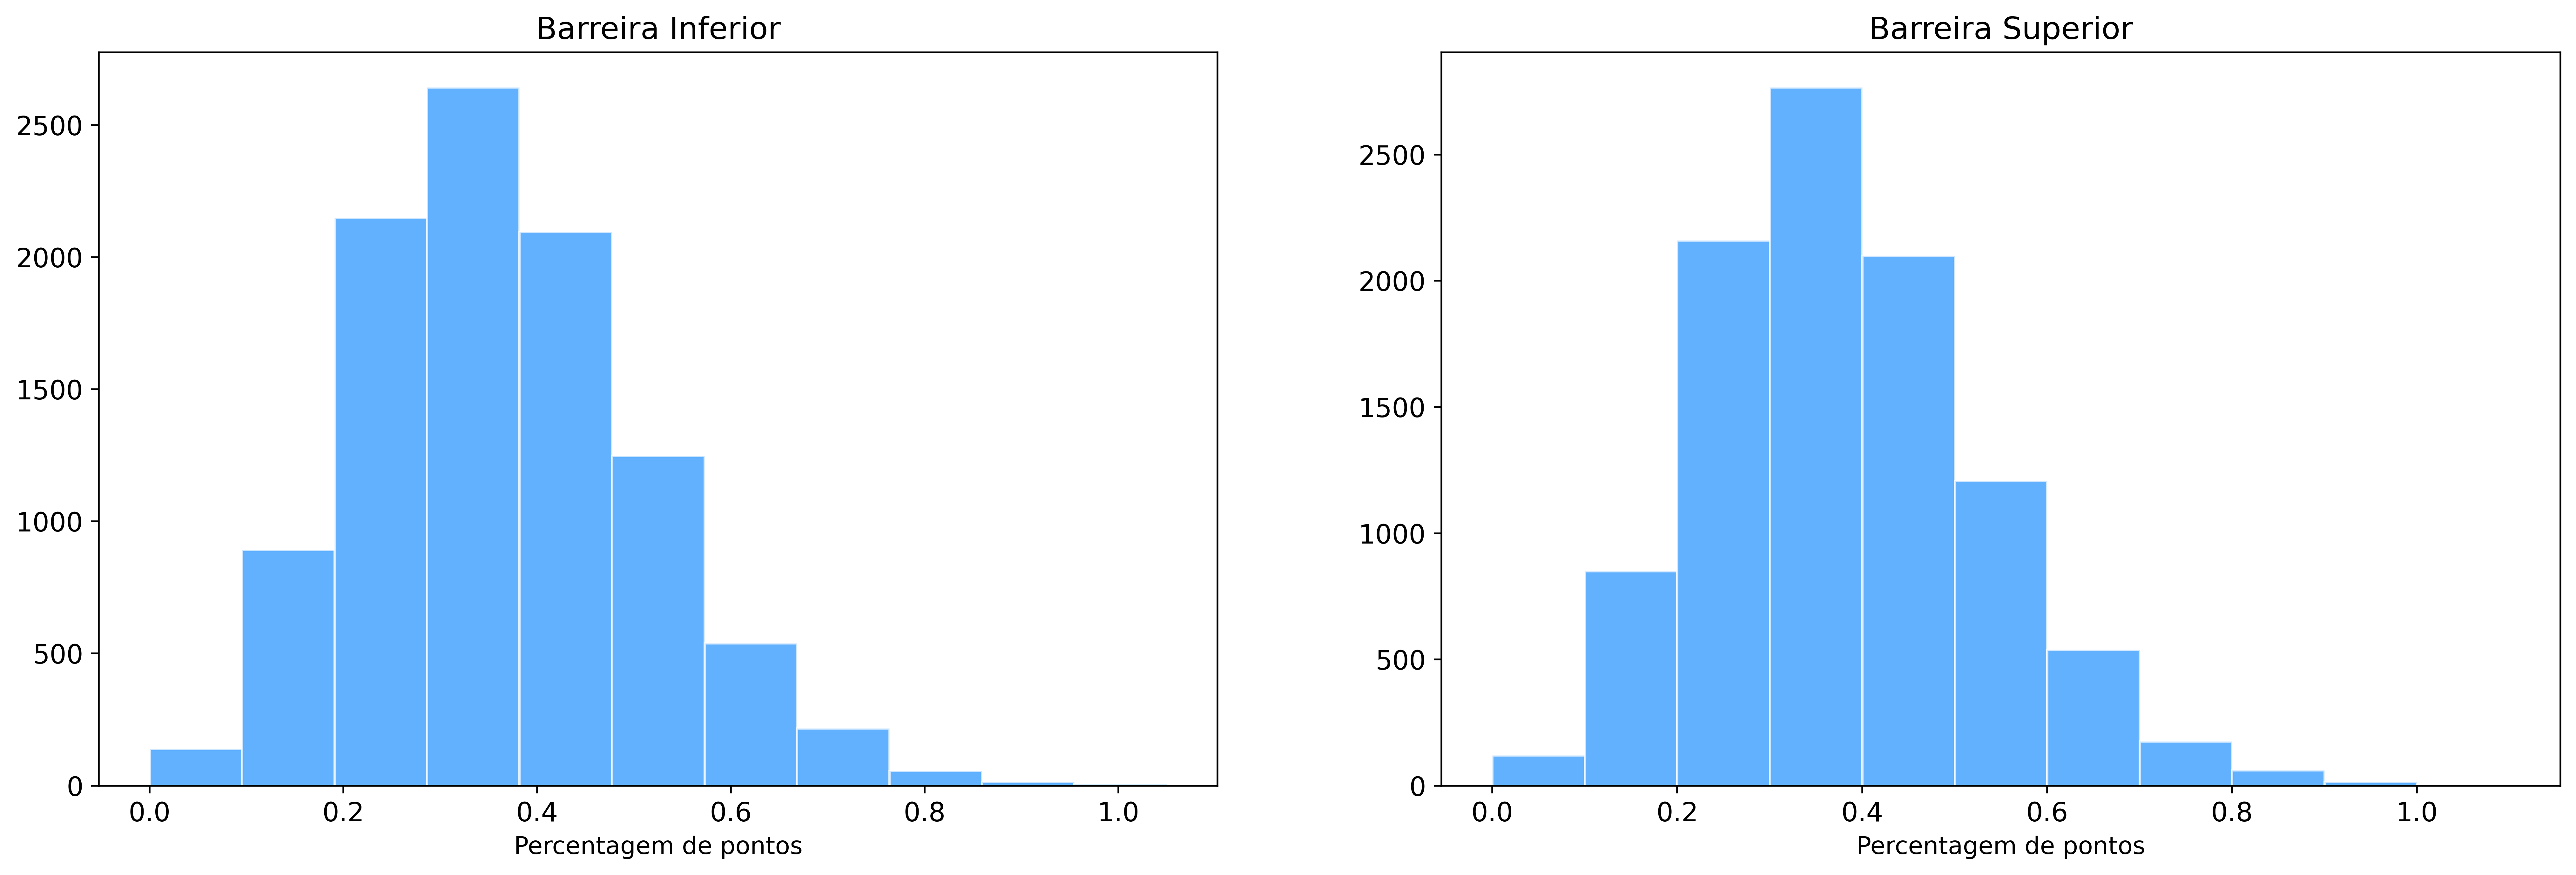
\includegraphics[width=\textwidth]{imagens/stats/histos_barreiras.png}
	\caption{Distribuição da percentagem de outliers, para ambos os lados da distribuição, de 10000 amostras geradas a partir de uma distribuição normal.}
	\label{fig:normalouts}
\end{figure}







\chapter{Construção das \textit{Red Flags}}

\begin{code}[caption={\textit{Query} em PostgreSQL para detetar contratos cuja data de publicação do anúncio em Diário da República seja feito num domingo ou feriado nacional.},captionpos=b, label=lst:rf3code,
	language=SQL,
	showspaces=false,
	basicstyle=\ttfamily,
	numbers=left,
	numberstyle=\tiny,
	commentstyle=\color{gray},	frame=single,
	breaklines=true,
	autogobble = true,
	postbreak=\mbox{\textcolor{red}{$\hookrightarrow$}\space},
	]
	WITH sundays AS (
		SELECT generate_series::date AS sunday_date
		FROM generate_series('2018-01-01'::date, '2024-05-01'::date, '1 week'::interval)
		WHERE EXTRACT(DOW FROM generate_series) = 0)
	SELECT contratos_basegov."id"
	FROM contratos_basegov
	JOIN concursos_publicos ON contratos_basegov."id" = concursos_publicos."id"
	WHERE tipo_procedimento = 'Concurso público' 
		AND EXTRACT(YEAR FROM contratos_basegov."data_publicacao") >= 2018 
		AND contratos_basegov."data_celebracao" <= '2024-05-01'
		AND (TO_CHAR(contratos_basegov."anuncio_drPublicationDate", 'MM-DD') IN 
		('01-01','04-25','05-01','06-10','08-15','10-05','11-01','12-01','12-08','12-25')
		OR contratos_basegov."anuncio_drPublicationDate" IN (SELECT sunday_date FROM sundays));
	
\end{code}


\begin{figure}[H]
	\centering
	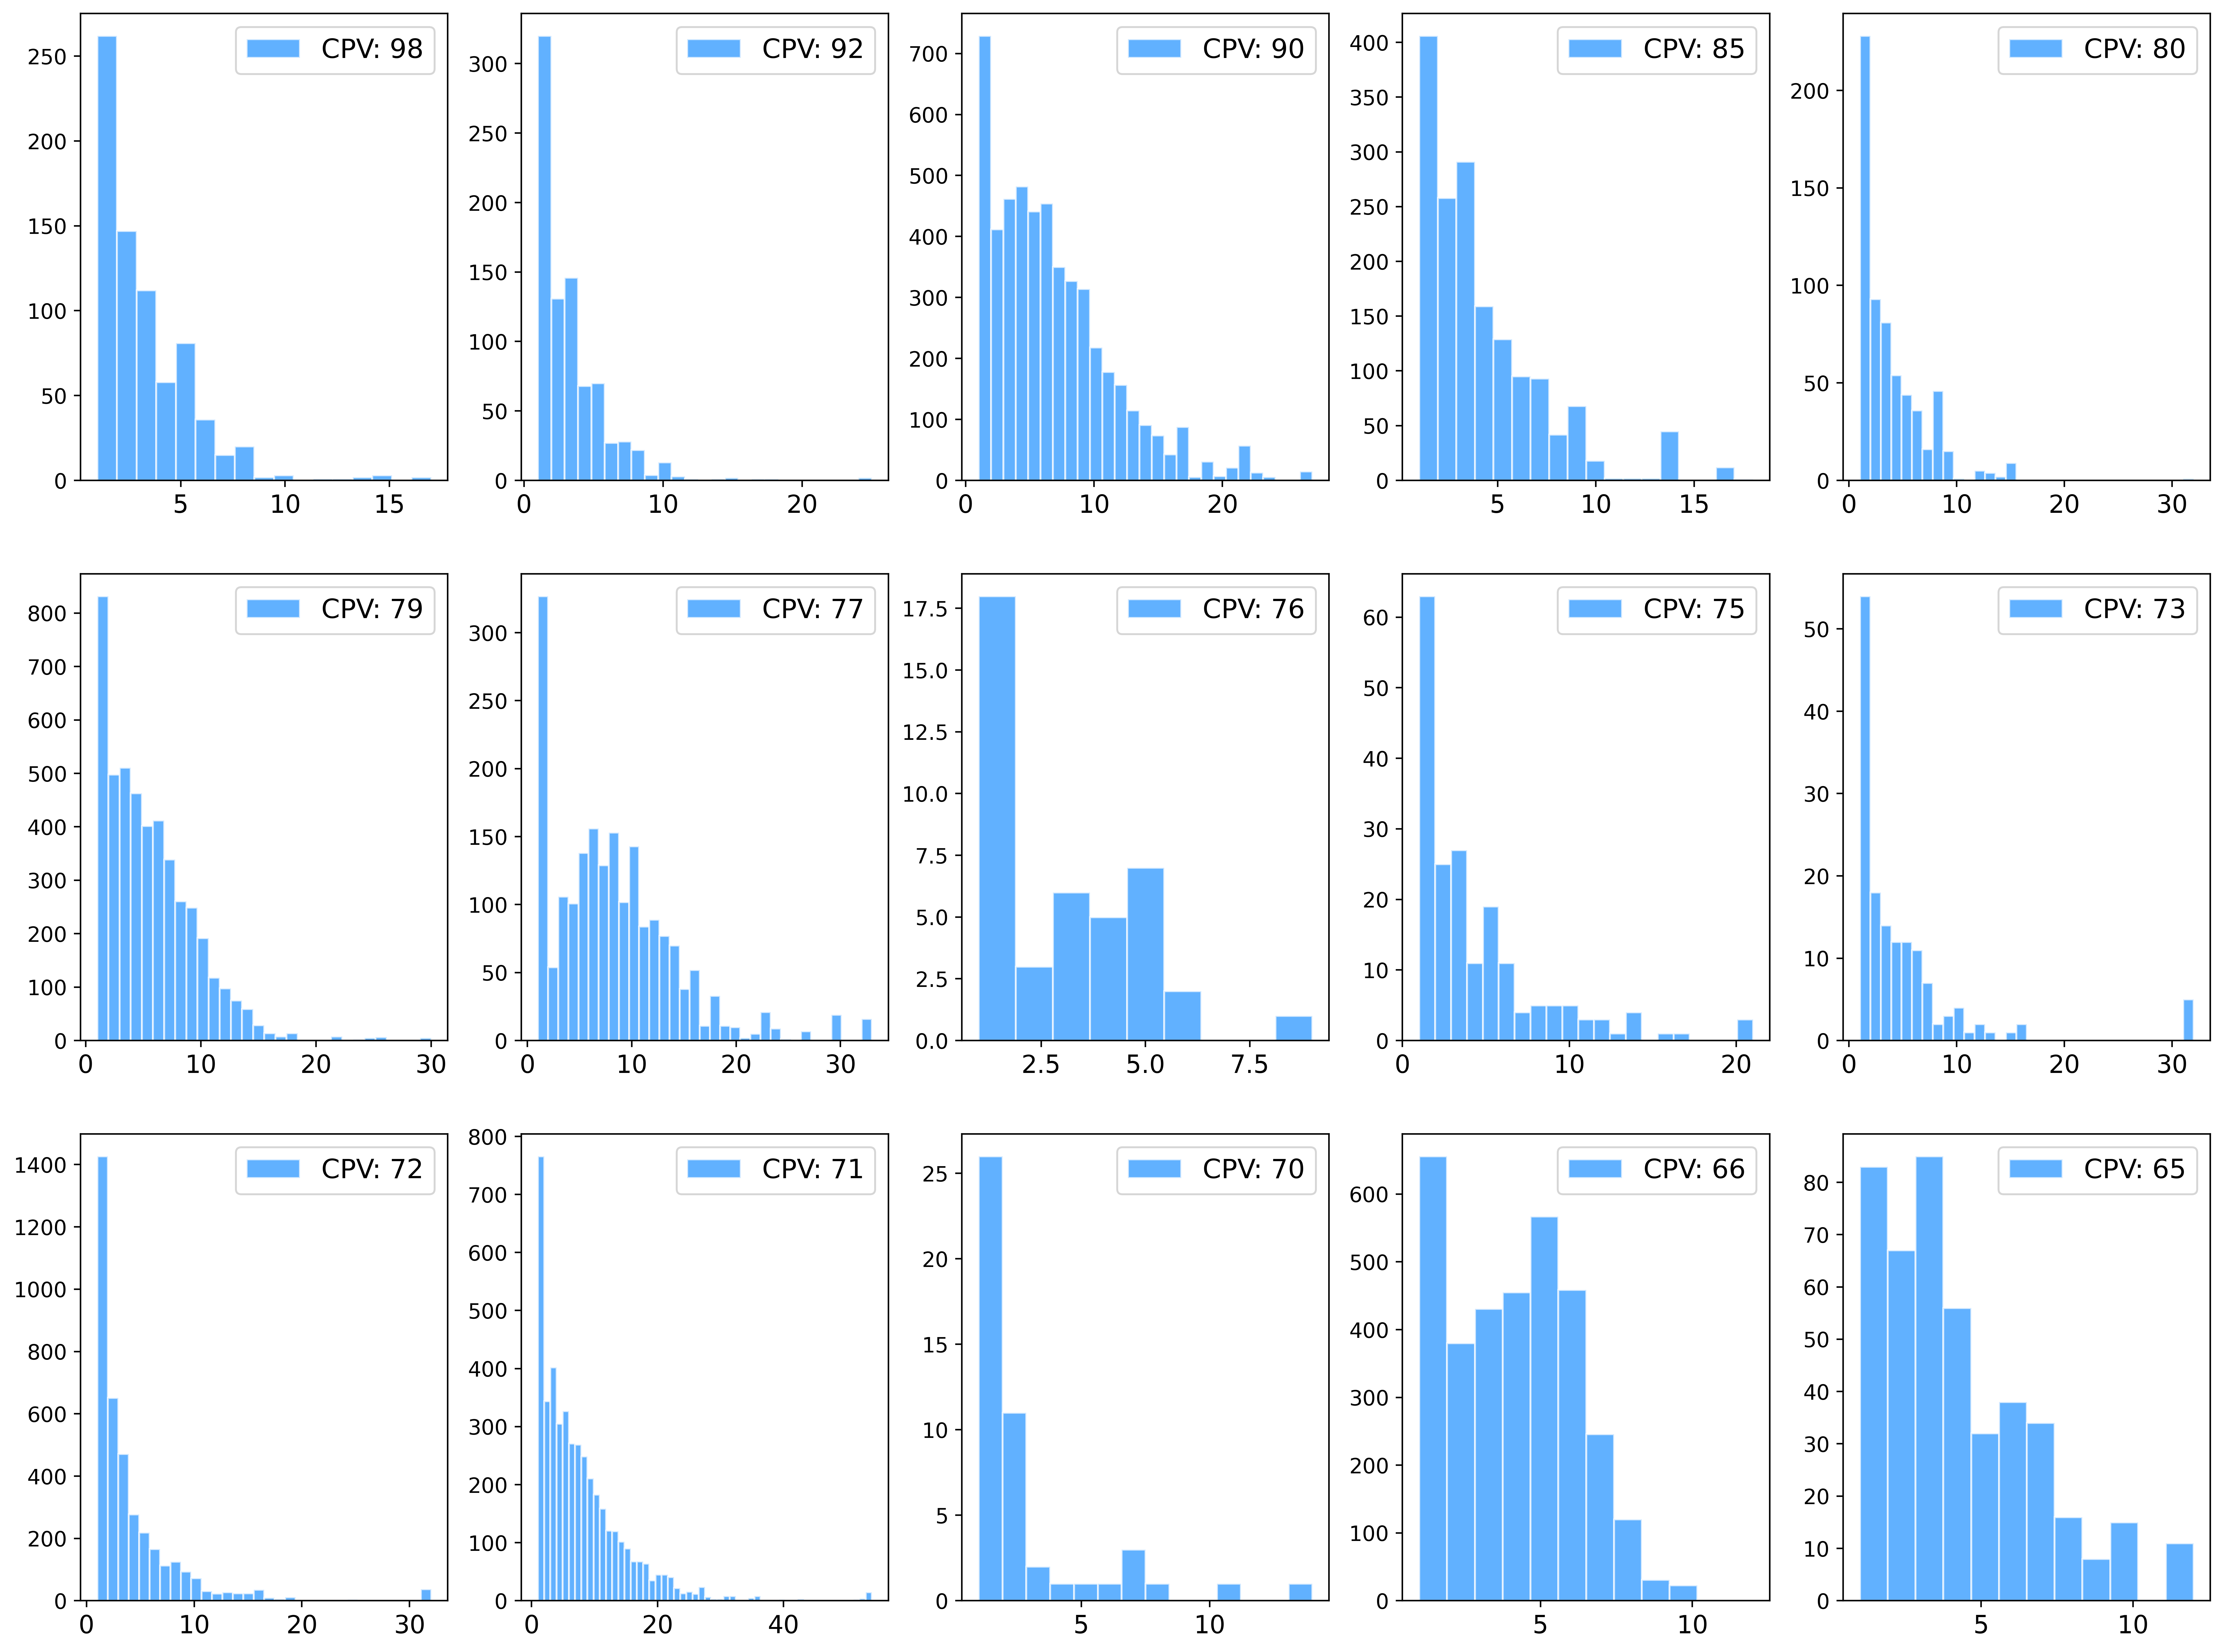
\includegraphics[width=\textwidth]{imagens/r019_hist1.png}
\end{figure}

\begin{figure}[H]
	\centering
	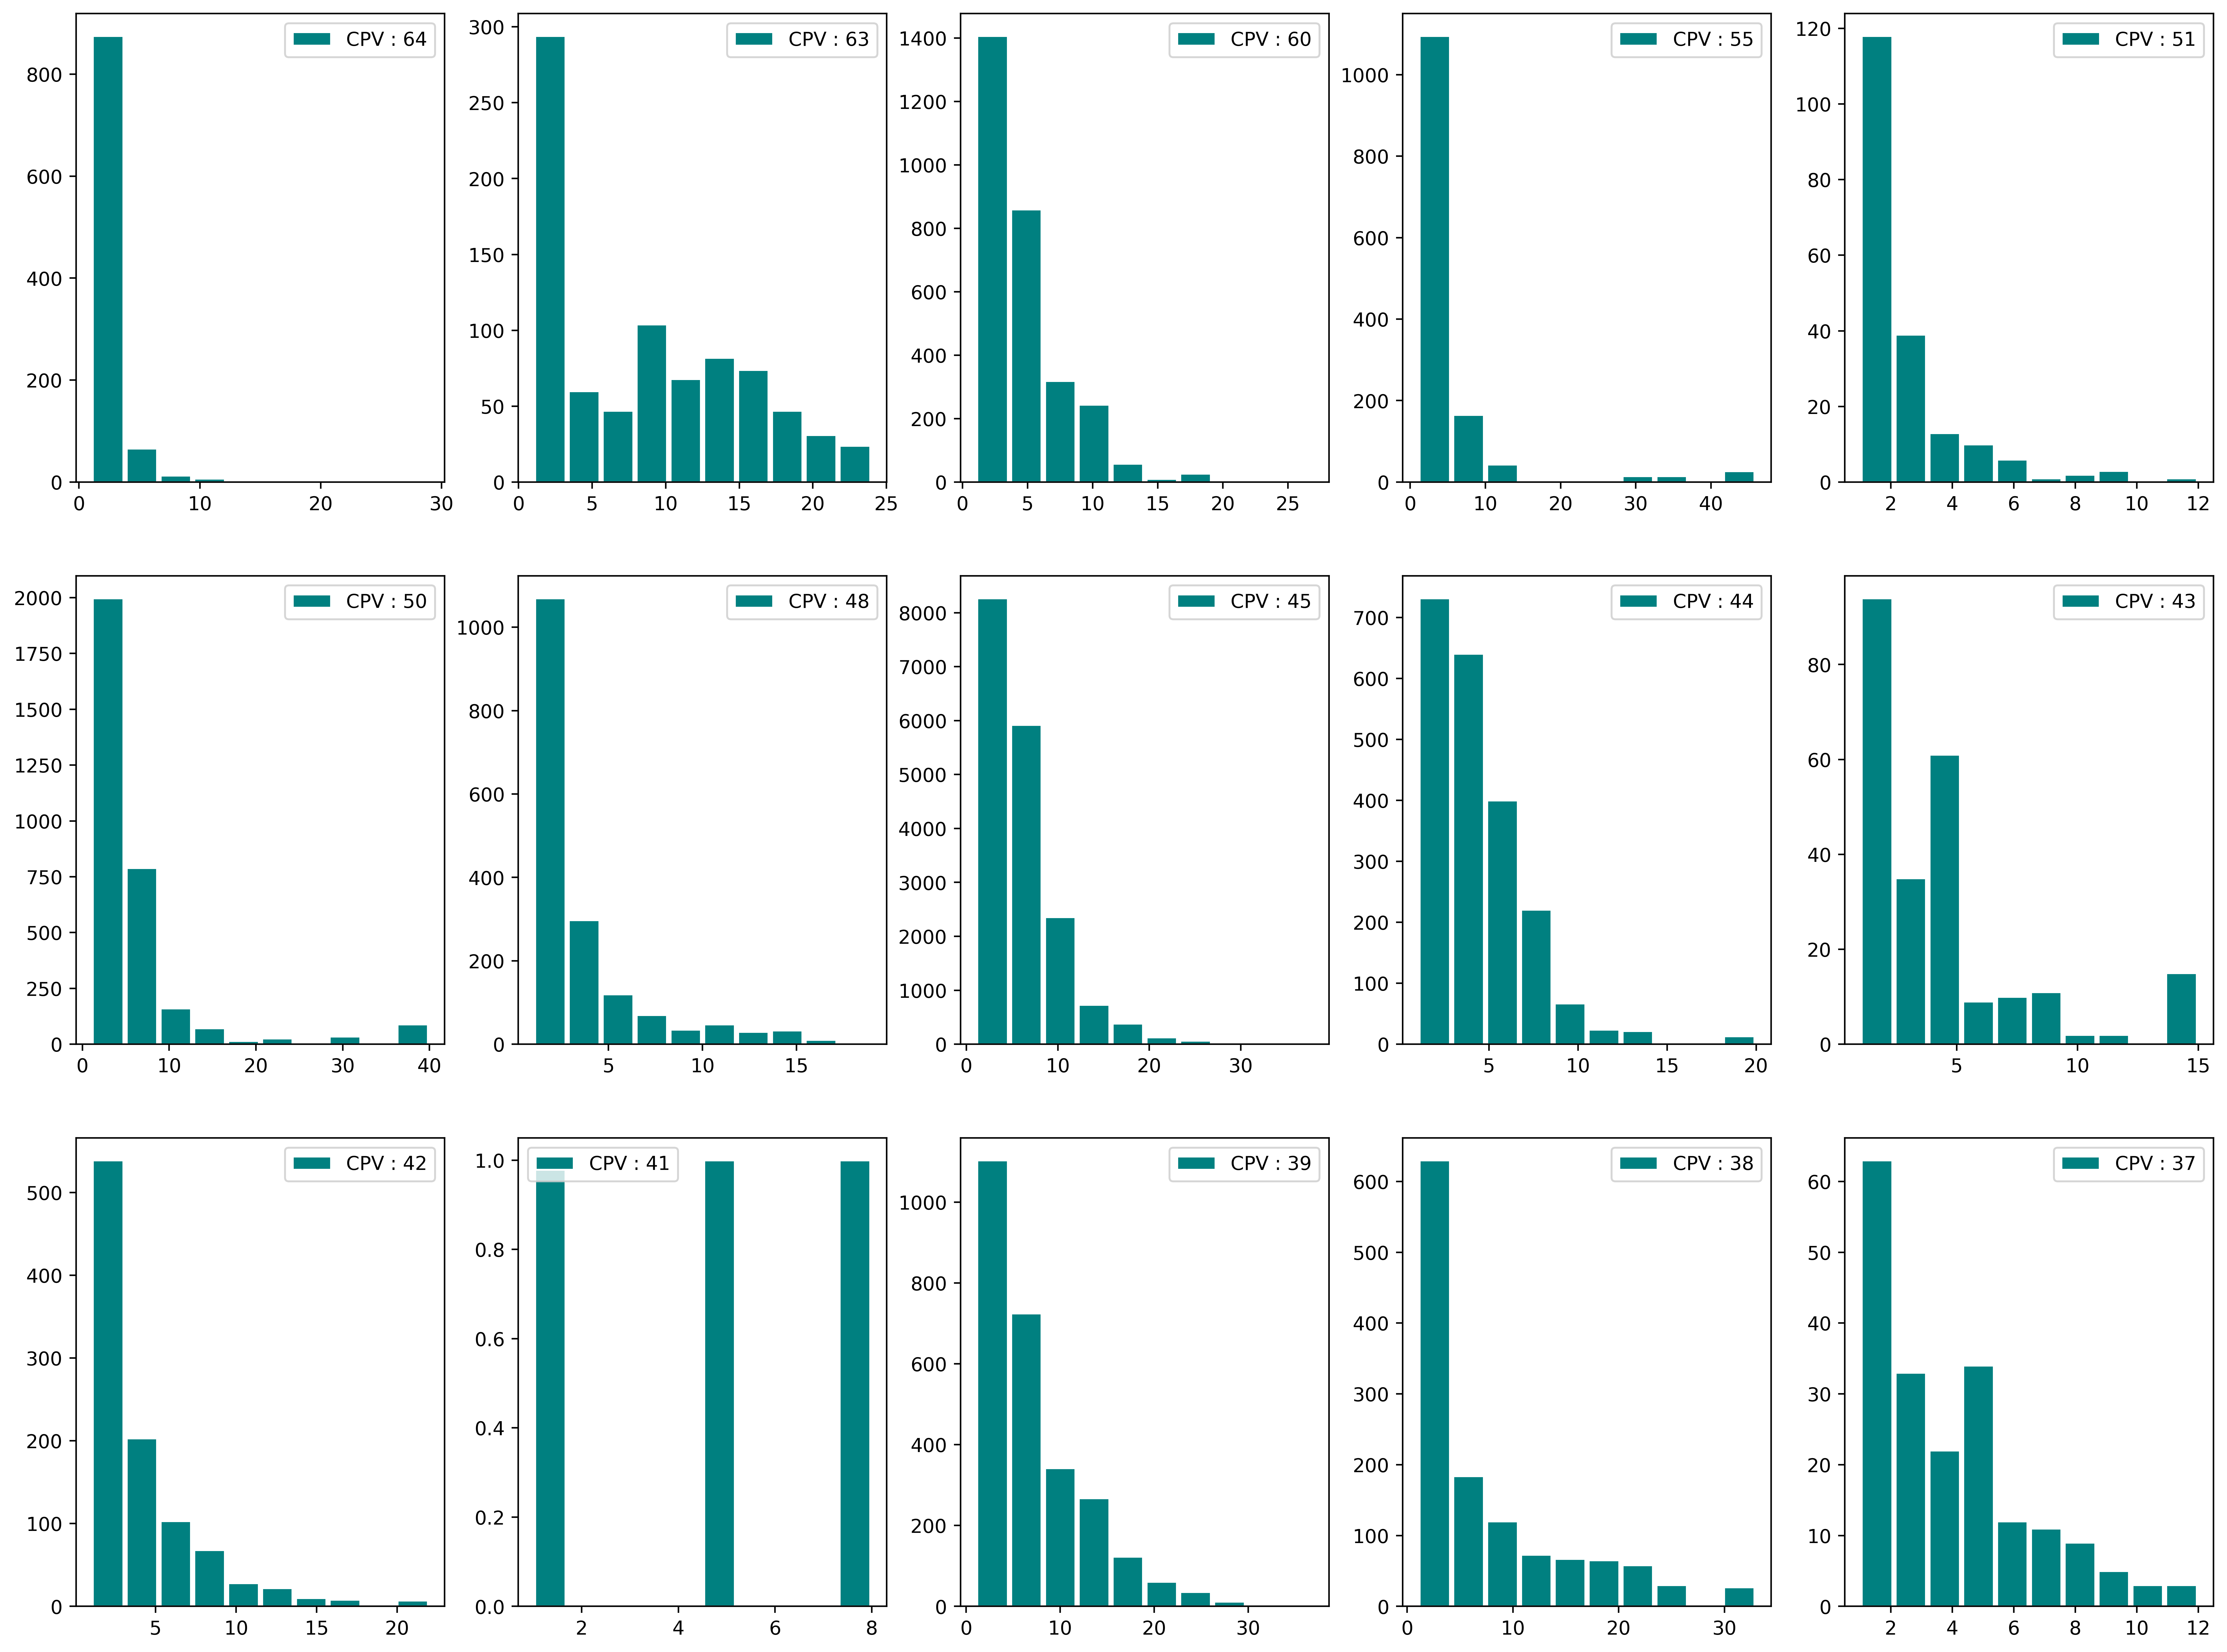
\includegraphics[width=\textwidth]{imagens/r019_hist2.png}
\end{figure}

\begin{figure}[H]
	\centering
	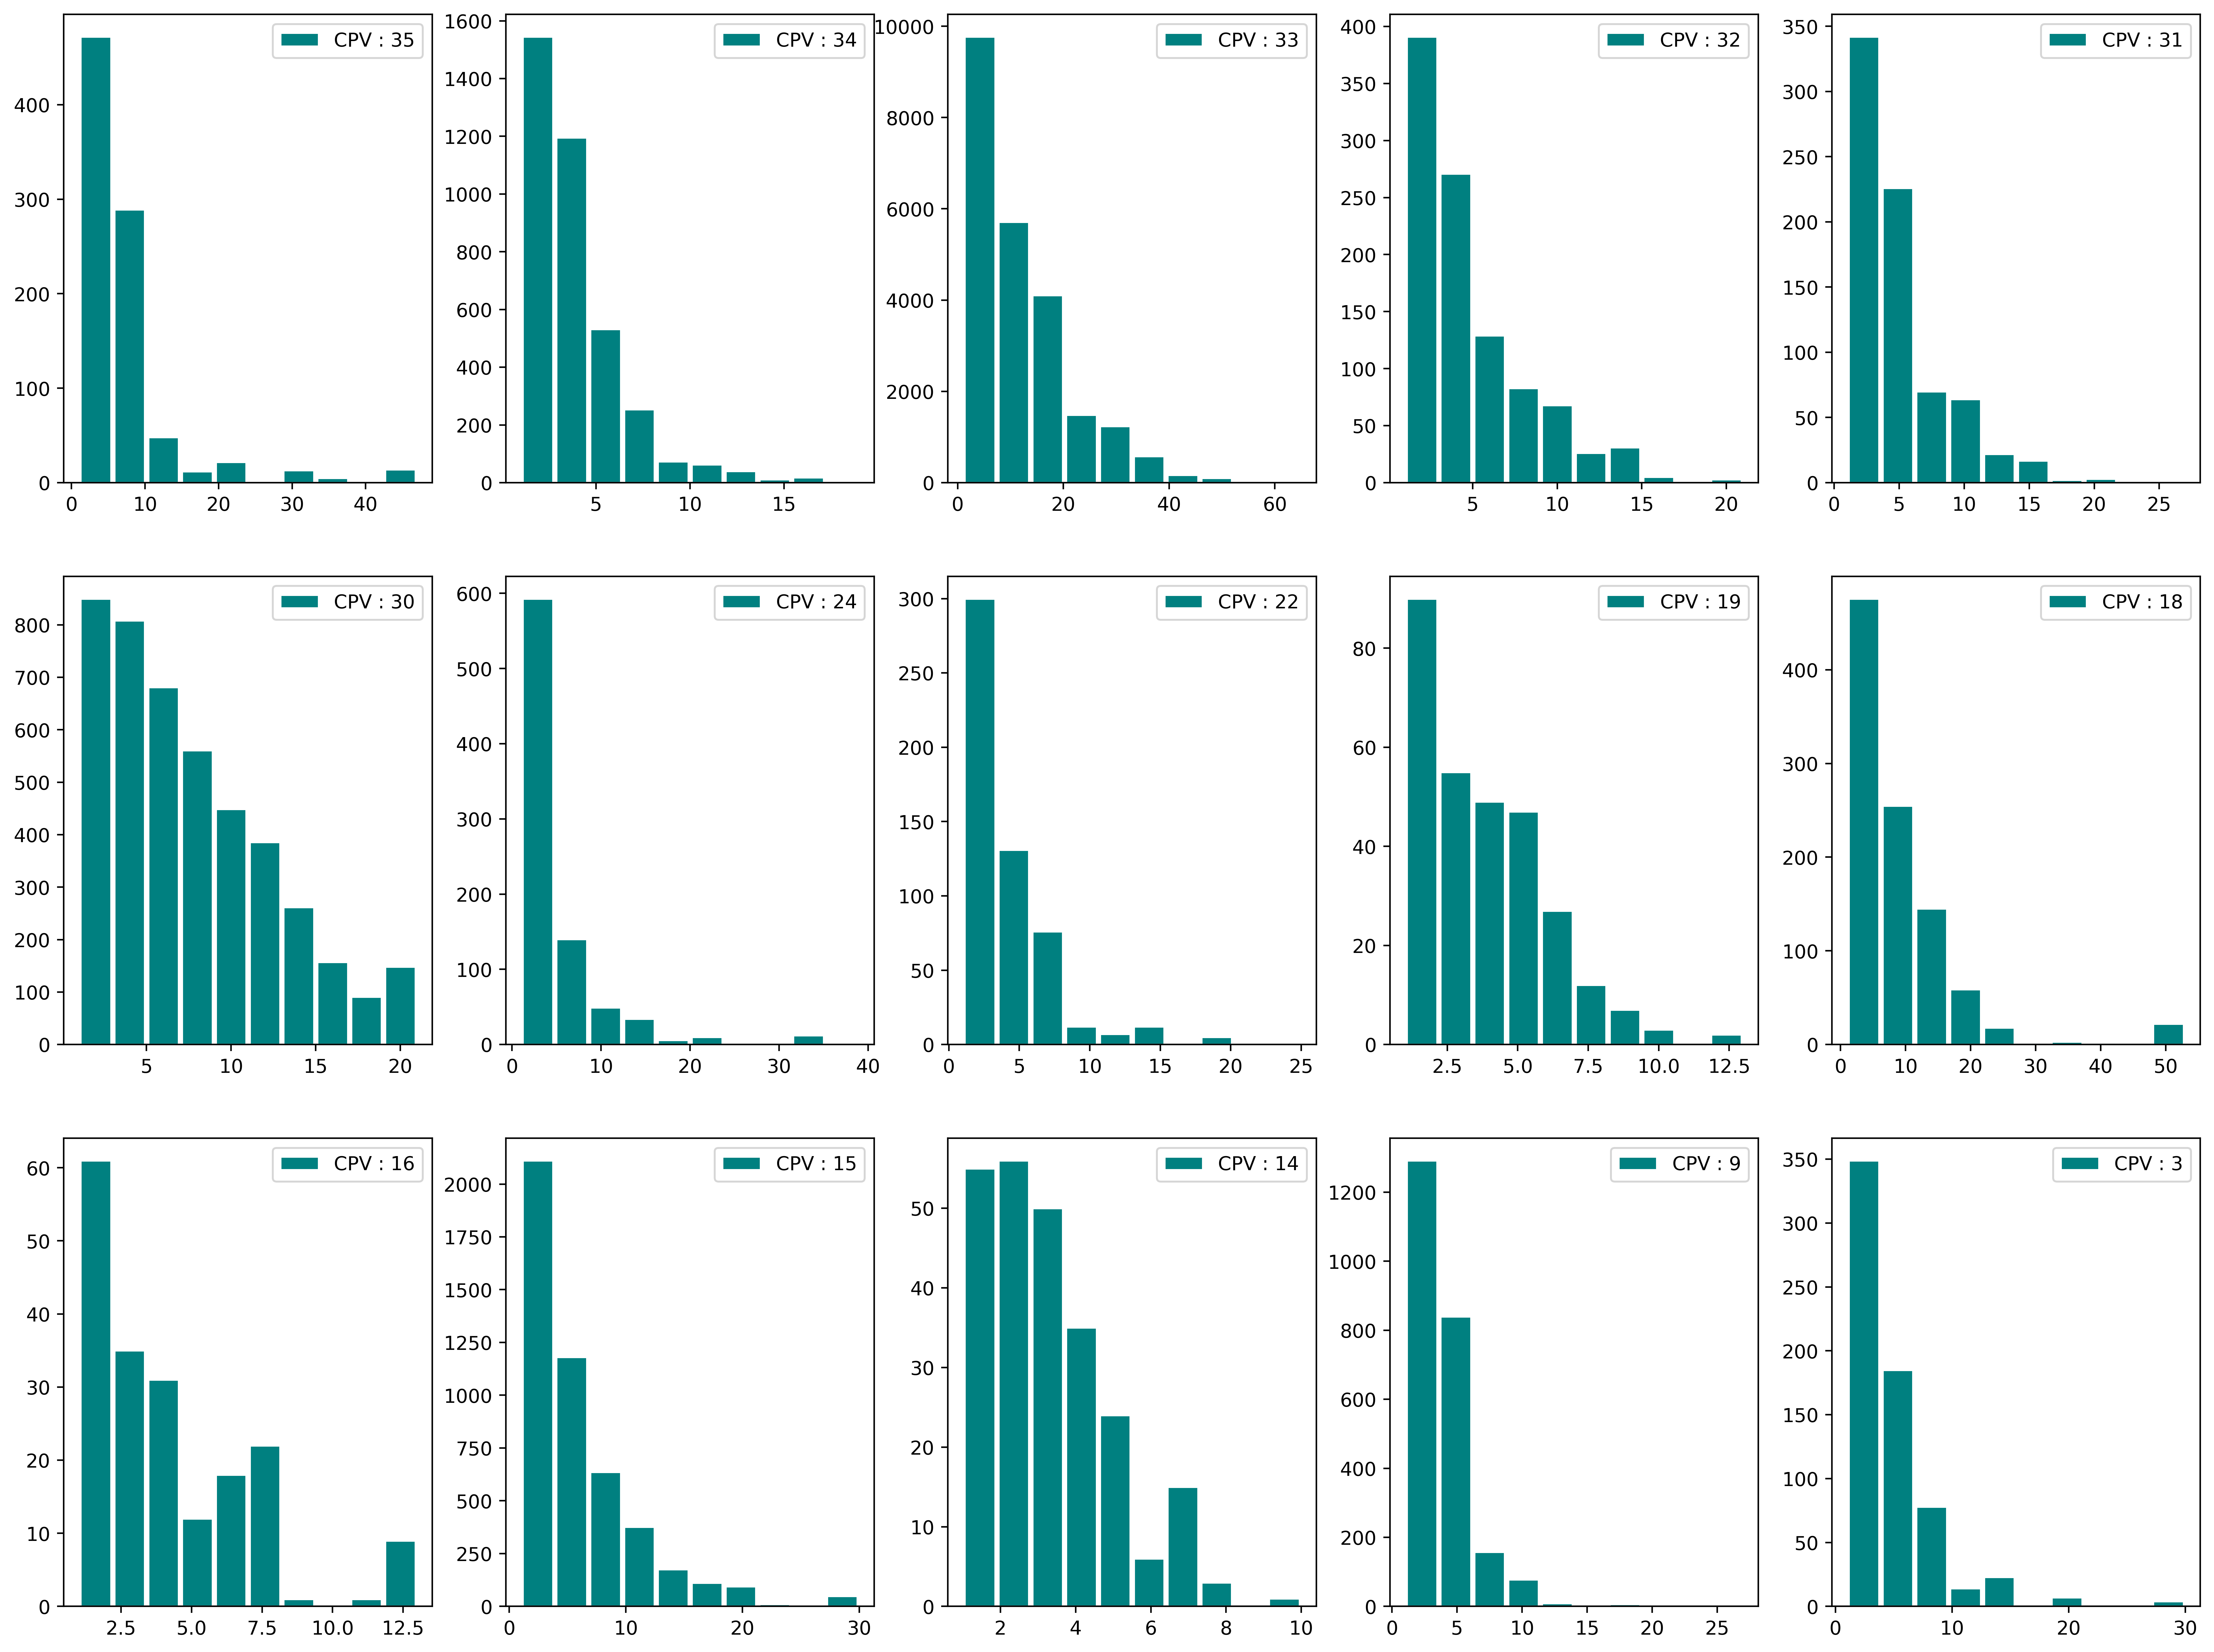
\includegraphics[width=\textwidth]{imagens/r019_hist3.png}
	\caption{Distribuição do número de entidades concorrentes por cada umas das 45 divisões de CPV.}
	\label{fig:distisnec}
\end{figure}

\begin{figure}[H]
	\centering
	\includegraphics[width=\textwidth]{imagens/cpv3.png}
	\caption{Boxplot do número de entidades concorrentes por cada umas das 45 divisões de CPV.}
	\label{fig:boxplotsnec}
\end{figure}


\begin{code}[caption={Código em Python referente à flag R031.},captionpos=b,label=lst:r31,
	language=python,
	showspaces=false,
	showstringspaces=false,
	basicstyle=\ttfamily,
	numbers=left,
	numberstyle=\tiny,
	commentstyle=\color{gray}, 
	frame=single,
	autogobble=true,
	breaklines=true,
	postbreak=\mbox{\textcolor{red}{$\hookrightarrow$}\space},
	]
	def flagr31(tol):
		"""
		Parametro de entrada:
		tol(float): número entre 0 e 1
		
		return: tuplo de IDs que respeitam as condicoes impostas
		"""
	
		cur = conn.cursor()
		cur.execute('''
		SELECT id
		FROM contratos_basegov
		WHERE tipo_procedimento = 'Concurso publico' 
		AND anuncio_preco_base IS NOT NULL 
		AND anuncio_preco_base > 0 
		AND preco_contratual < anuncio_preco_base 
		AND preco_contratual > anuncio_preco_base * (1 - %s) 
		AND n_anuncio IN (
		SELECT n_anuncio
		FROM contratos_basegov
		GROUP BY n_anuncio
		HAVING COUNT(DISTINCT n_anuncio) = 1
		);
		''', (tol,))
	
		return(cur.fetchall())
	
\end{code}



\begin{figure}[h]
	\begin{minipage}{.33\textwidth}
		\centering
		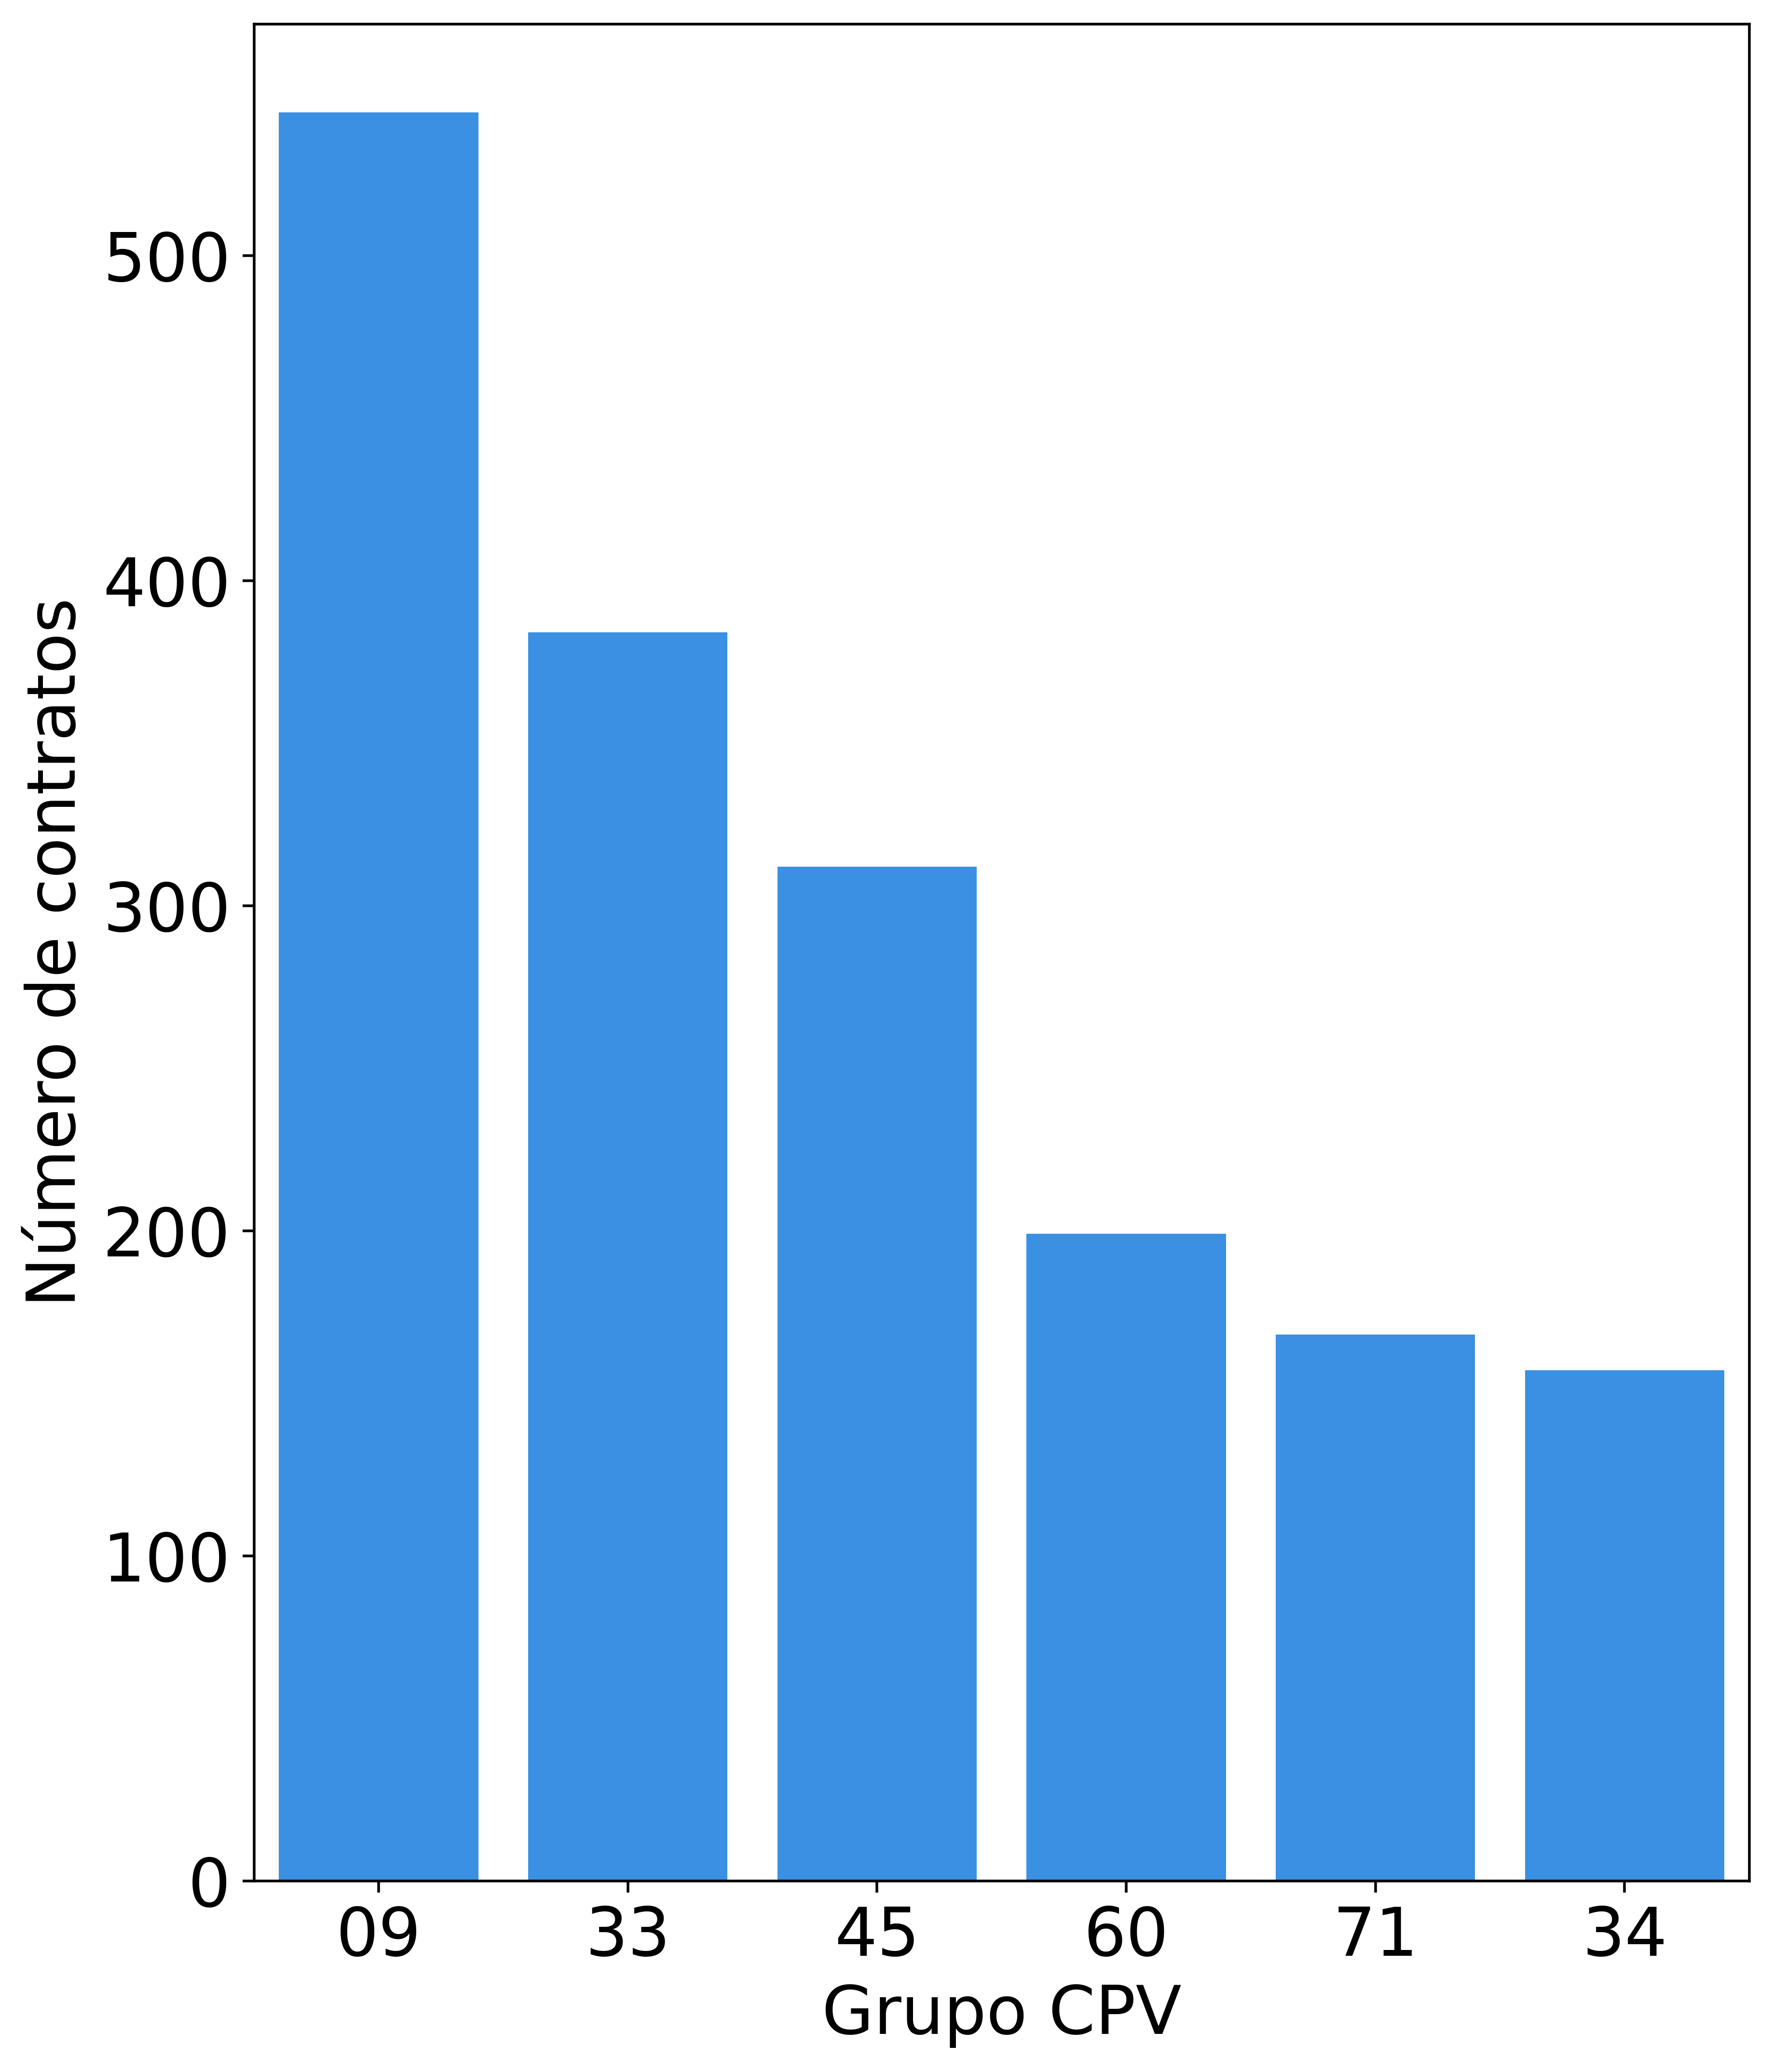
\includegraphics[width=1\linewidth]{imagens/r31/pb.png}
		\caption{Distribuição do número de concursos públicos, cujo valor do preço base no Portal BASE é nulo, por divisão de CPV.}
		\label{fig:r31nulos}
	\end{minipage}
	\begin{minipage}{.33\textwidth}
		\centering
		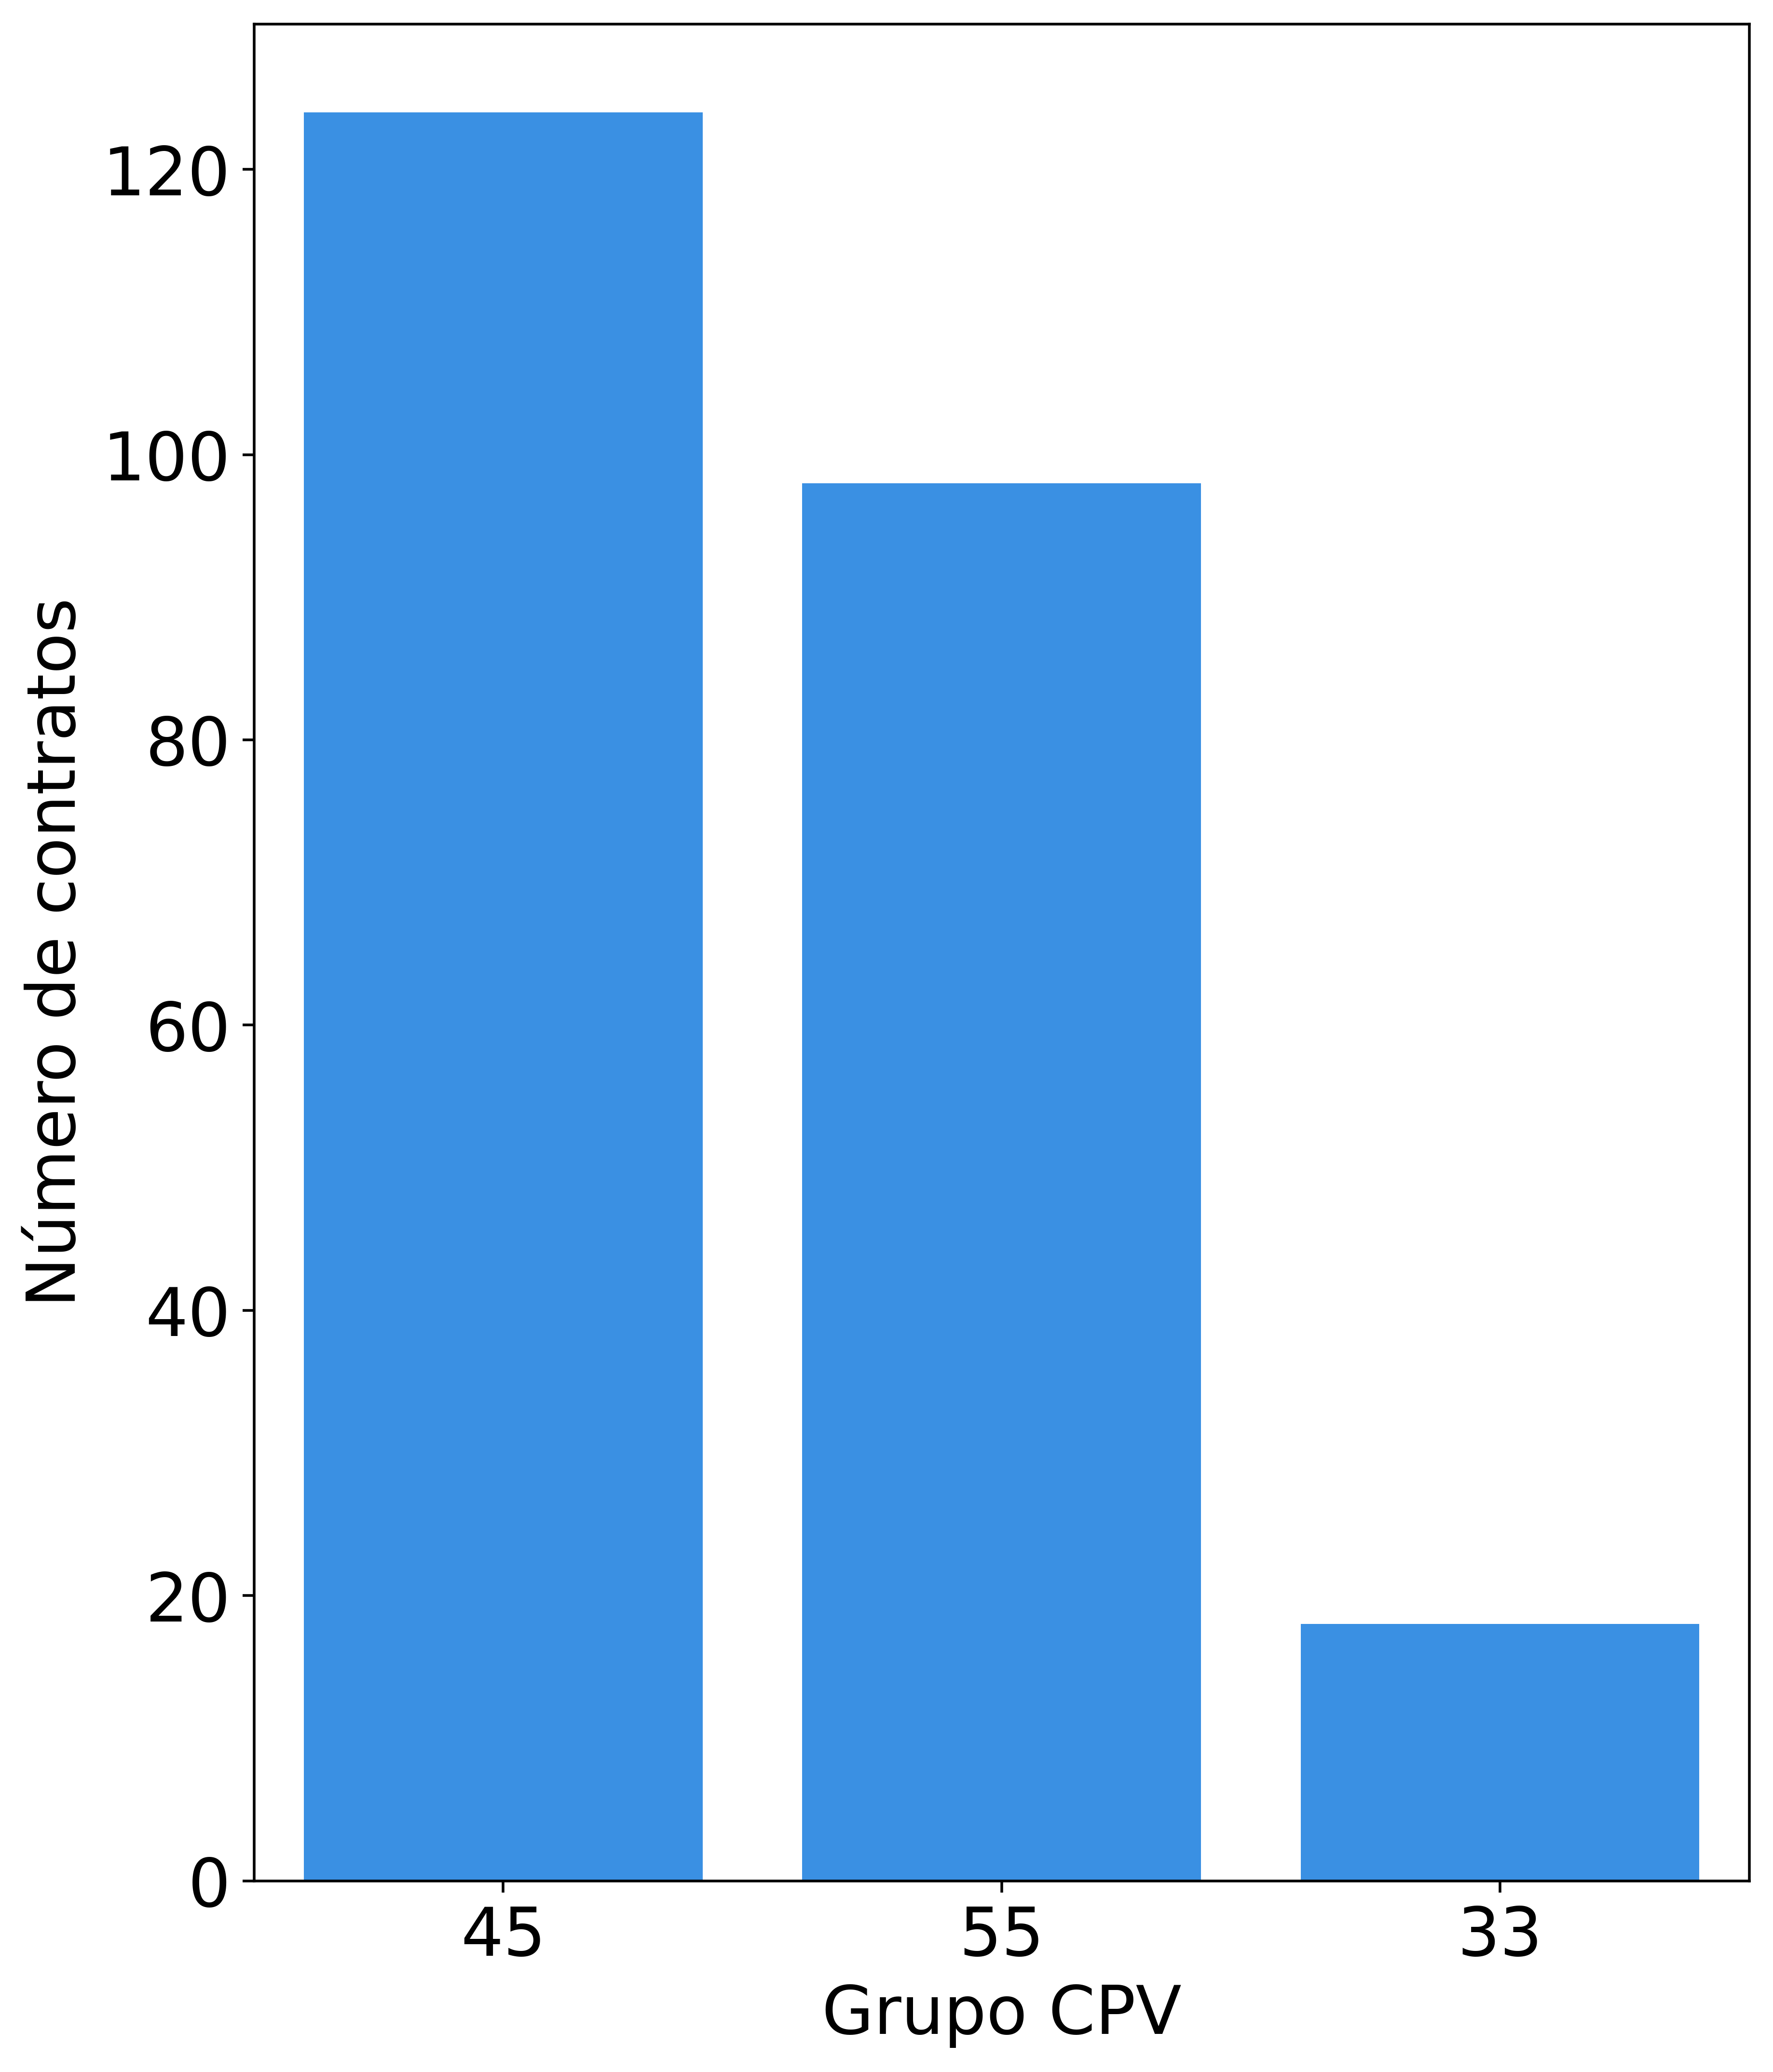
\includegraphics[width=1\linewidth]{imagens/r31/pcpb.png}
		\caption{Distribuição do número de concursos públicos, cujo valor do preço contratual é superior ao preço base, por divisão de CPV.}
		\label{fig:r31nulos2}
	\end{minipage}
	\begin{minipage}{.33\textwidth}
		\centering
		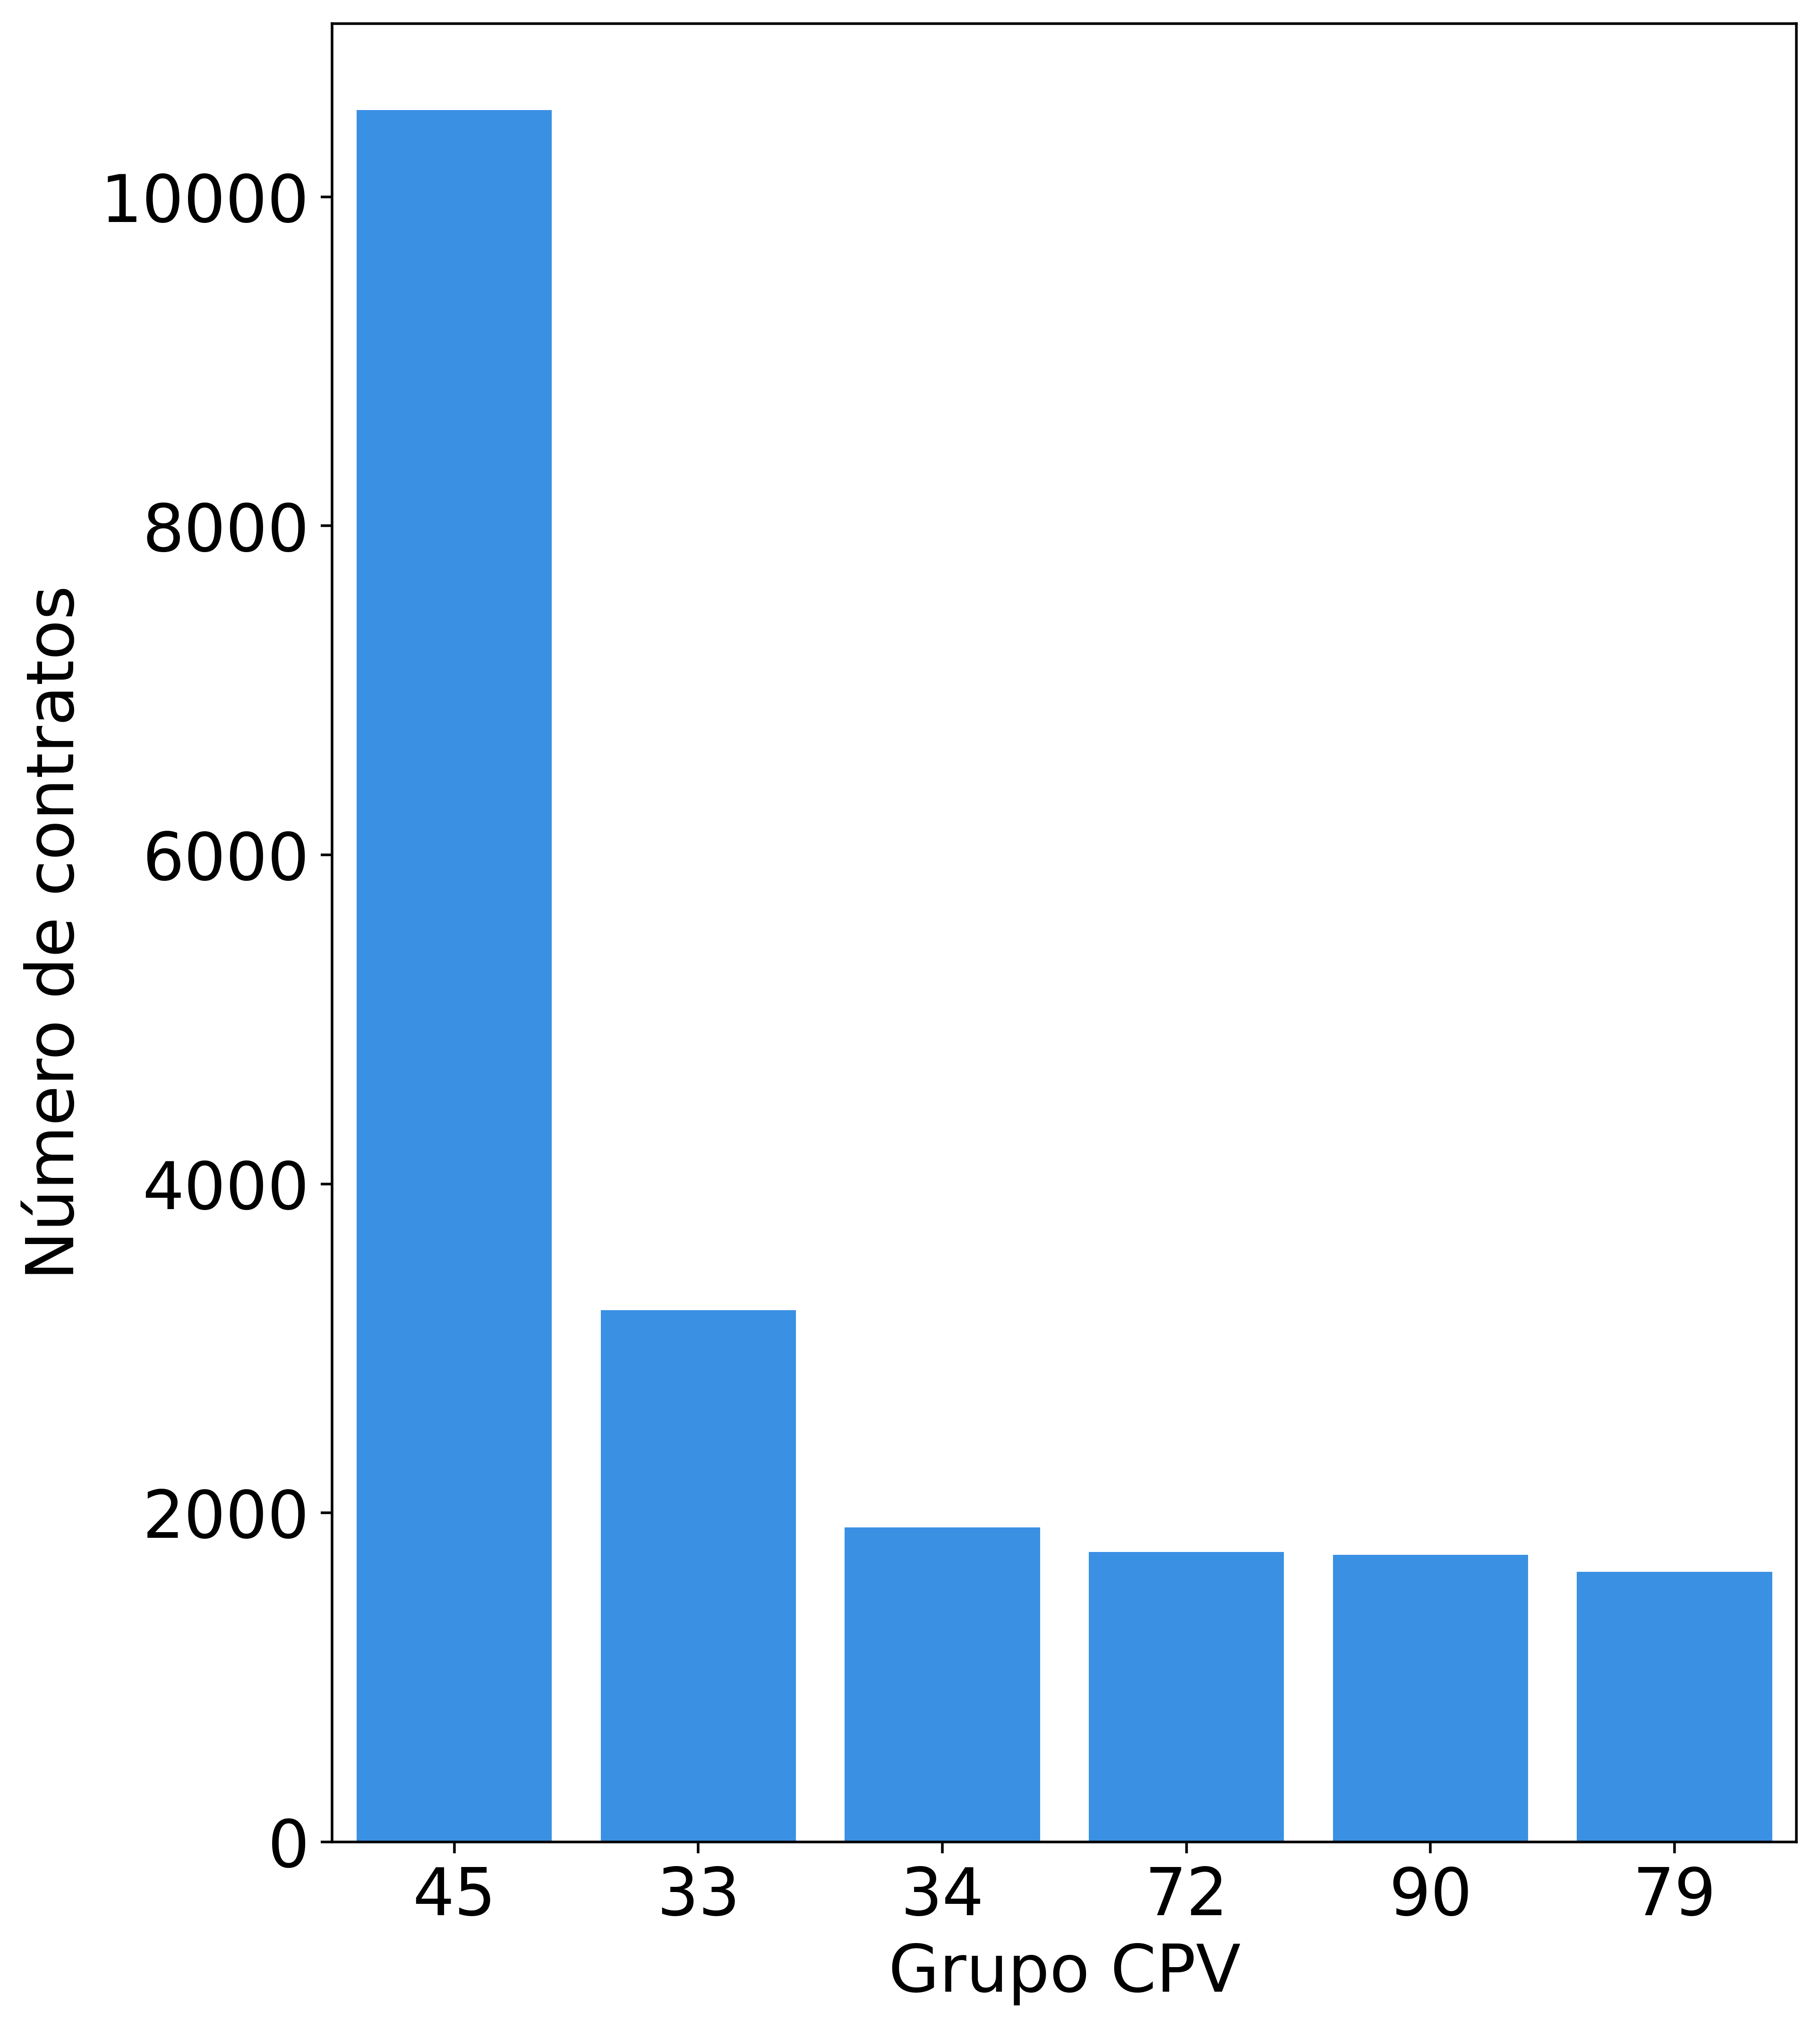
\includegraphics[width=1\linewidth]{imagens/r31/pcpbnear.png}
		\caption{Distribuição do número de concursos públicos, cujo valor do preço contratual é muito próximo do preço base, por divisão de CPV.}
		\label{fig:r31nulo3}
	\end{minipage}
\end{figure}

